\lecture{4}{20/1}

\begin{example}
    Integrate $f(x, y) = 4xy - y^3$ over $A$ where $A$ is the finite region
    between $y = x^3$ and $y = \sqrt x$ for $x \in [0, 1]$.
\end{example}

\begin{figure}[]
    \centering
    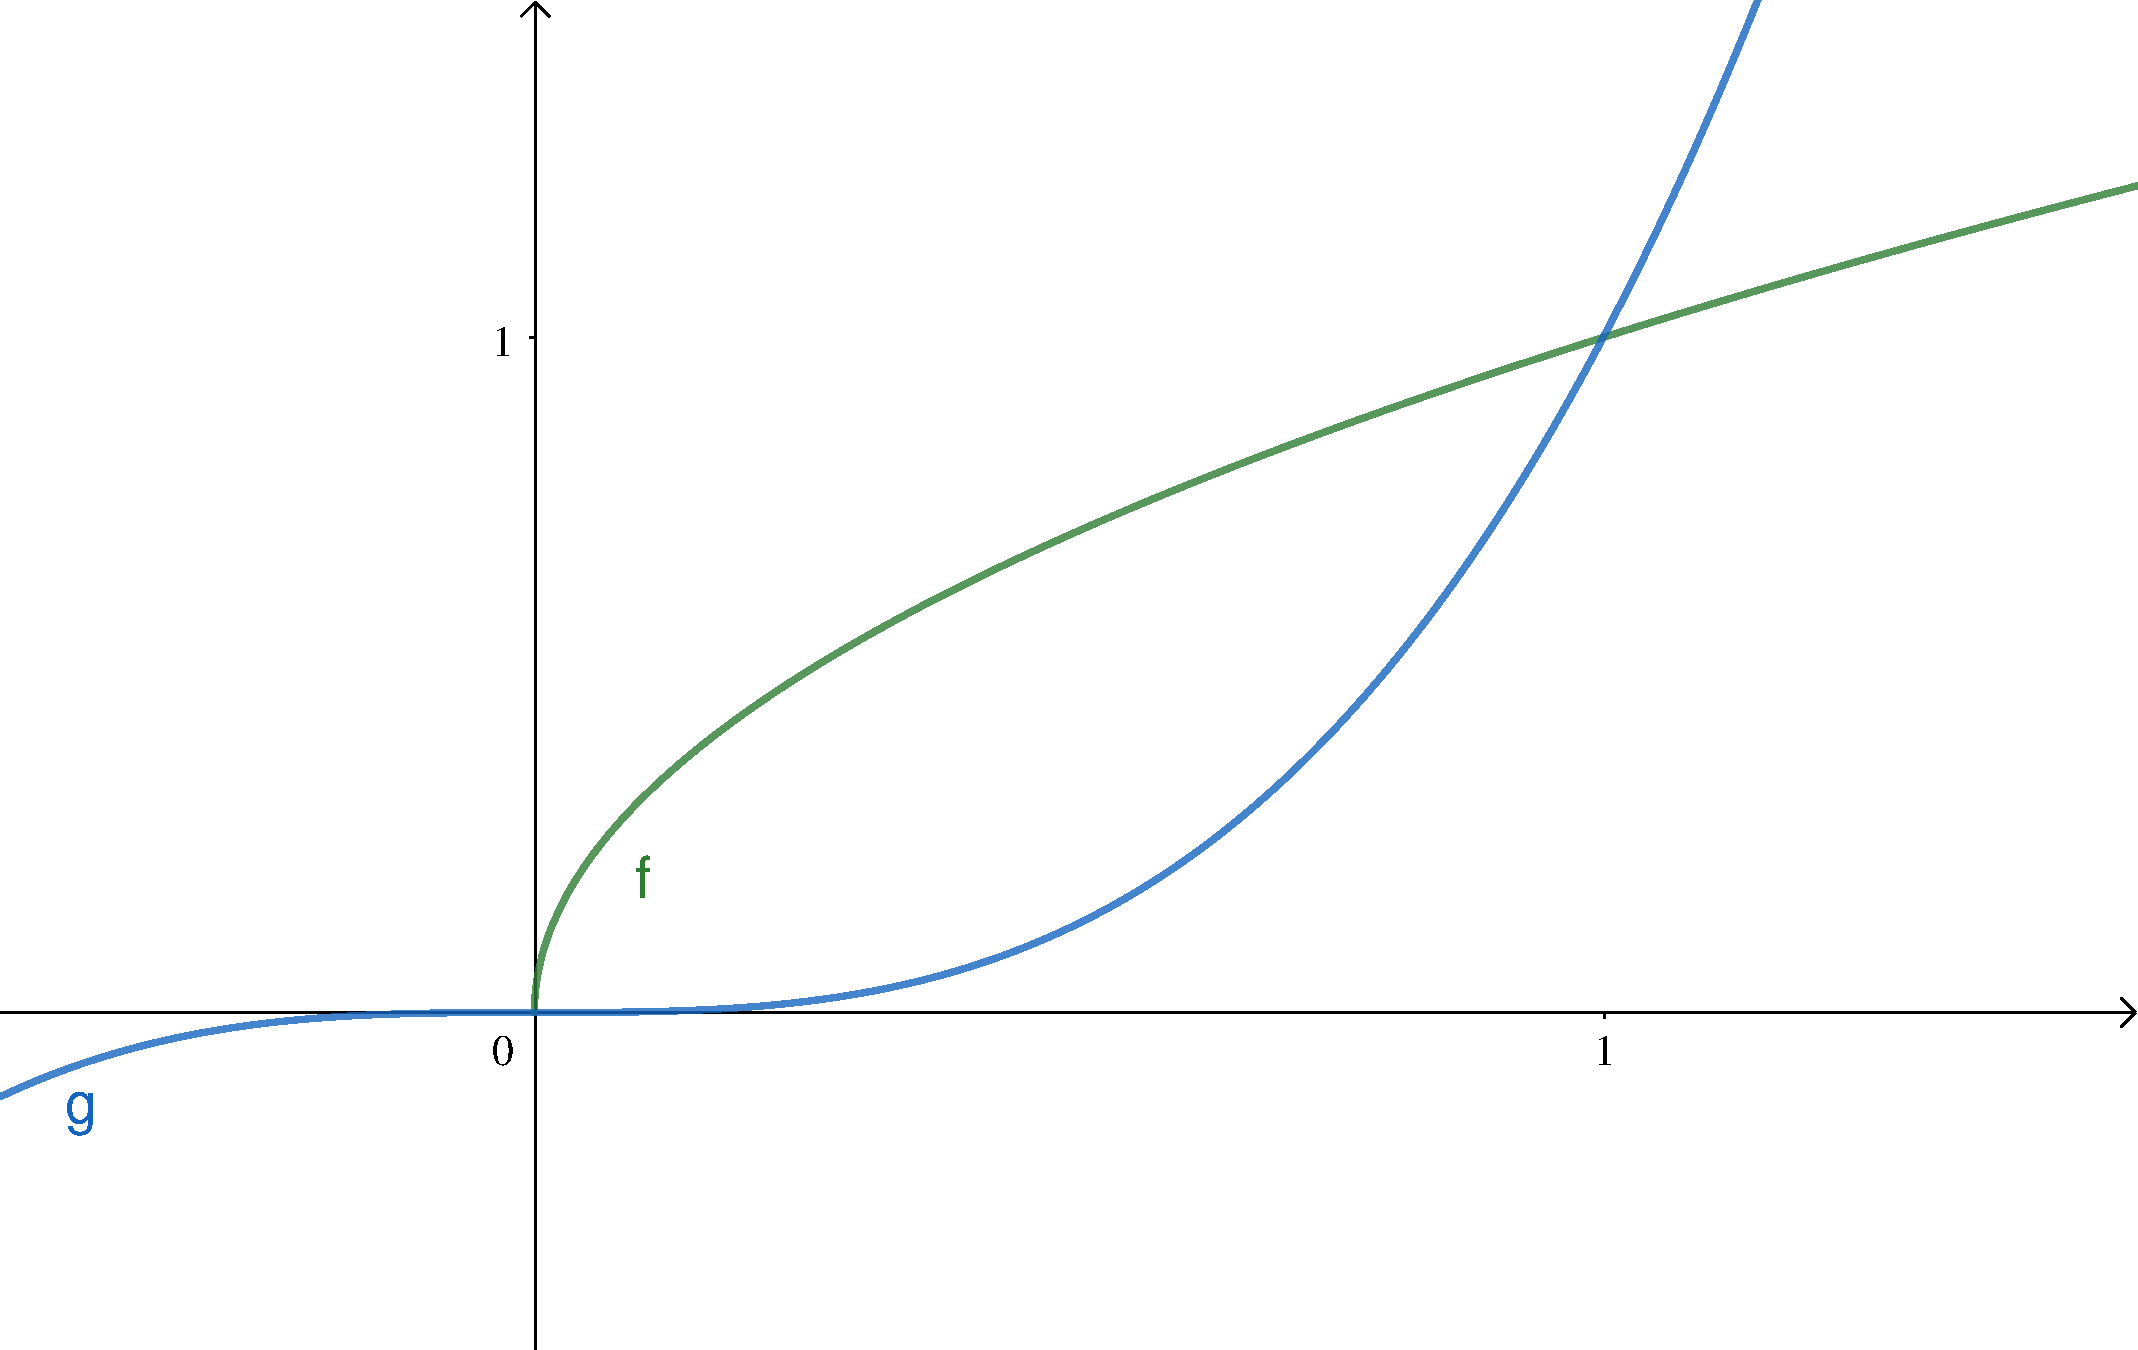
\includegraphics[width=0.8\linewidth]{images/fubini-ex-1.pdf}
    \caption{}
    \label{fig:fubini-ex-1}
\end{figure}

\begin{solution}
    The first thing we should do is draw $A$, as shown in Figure 
    \ref{fig:fubini-ex-1}.
    So we have
    \begin{align*}
        \int_A (4xy - y^3) \, dA
        &= \int_0^1 \int_{x^3}^{\sqrt x} (4xy - y^3) \, dy \, dx \\
        &= \int_0^1 \left(2xy^2 - \frac14y^4\right)^{\sqrt x}_{x^3} \, dx \\
        &= \int_0^1 (2x^2 - \frac14x^2 - 2x^7 + \frac14x^{12}) \, dx \\
        &= \left(\frac23x^3 -\frac1{12}x^3 - \frac14x^8 + 
            \frac1{52}x^{13}\right)_0^1 \\
        &= \frac23 - \frac1{12} - \frac14 + \frac1{52} = \frac{55}{156}.
    \end{align*}
    As the region $A$ is $x$-simple and $y$-simple,
    you can swap the order of integration and still get the same answer.
\end{solution}

\begin{example}
    Integrate $f(x, y) = e^{-x^2}$ over the triangle $A$ with
    vertices $(0,0)$, $(1,0)$, and $(1, 1)$.
\end{example}

\begin{solution}
    $A$ is clearly $x$-simple and $y$-simple, 
    so the order of integration does not matter.
    \begin{enumerate}
        \item 
            First attempt: we will attempt to integrate $x$ first.
            \[
                \int_A e^{-x^2} \, dA = \int_0^1 \int_y^1 e^{-x^2} \, dx \, dy;
            \]
            however, the antiderivative of $e^{-x^2}$ cannot be represented
            in terms of elementary functions.

        \item Second attempt: we will attempt to integrate $y$ first.
            \begin{align*}
                \int_A e^{-x^2} \, dA
                &= \int_0^1 \int_0^x e^{-x^2} \, dy \, dx \\
                &= \int_0^1 \left(ye^{-x^2}\right)^x_0 \, dx \\
                &= \int_0^1 \left(xe^{-x^2}\right) \, dx \\
                &= \left(-\frac12e^{-x^2}\right)^1_0 \\
                &= -\frac12e^{-1} + \frac12 \\
                &= \frac12\left(1-\frac1e\right).
            \end{align*}
    \end{enumerate}
\end{solution}

\begin{example}
    Integrate $f(x, y) = x^2 + y^2$ over $A = B_1(\bm 0)$.
\end{example}

\begin{solution}
    \begin{align*}
        \int_A(x^2 + y^2) \, dA
        &= \int_0^{2\pi} \int_0^1 r^2 \cdot r \, dr \, d\theta \\
        &= \int_0^{2\pi} \left(\frac14r^4\right)^{r = 1}_{r = 0} d\theta \\
        &= \int_0^{2\pi} \frac14 \, d\theta \\
        &= \left(\frac14\theta\right)^{2\pi}_0 = \frac{\pi}2
    \end{align*}
\end{solution}

\begin{example}
    Find the mass $M$ of air inside a hemispherical volume
    of radius $r$ centered at the origin, when the air density
    varys with height as $\rho = cz + \rho_0$ 
    ($c, \rho_0$ are constants).
\end{example}

\begin{solution}
    \begin{align*}
        M &= \int_0^r \int_{-r_z}^{r_z} 
        \int_{-\sqrt{r_z^2 - y^2}}^{\sqrt{r_z^2 - y^2}} \rho(z) \,dx\,dy\,dz \\
        \vdots \\
        M &= \int_0^r (cz + \rho_0) \pi (r^2 - z^2) \, dz \\
        \vdots \\
        M &= \pi \left( \frac c4 r^4 + \frac23 \rho_0 r^3 \right).
    \end{align*}
\end{solution}

\chapter{Line and surface integrals}
\section{Line integrals}

\begin{definition}[Regular arc]
    A \textbf{regular arc} is a parametrised curve $\bm x(t)$ for which
    the components $x_a(t)$ are continuous with continuous first derivatives,
    where $t$ lies in some (maybe infinite) interval $[\alpha, \beta]$.
\end{definition}

It is useful to consider \emph{regular curves} too, 
which is effectiveless just a series of regular arcs \emph{glued}
together.

\begin{definition}[Regular curve]
    A \textbf{regular curve} consists of a finite number of regular arcs
    joined end to end.
\end{definition}
